%% LyX 2.3.4.2 created this file.  For more info, see http://www.lyx.org/.
%% Do not edit unless you really know what you are doing.
\documentclass[english,dvipsnames,aspectratio=169,handout]{beamer}
\usepackage{mathptmx}
\usepackage{algorithm2e}
\usepackage{eulervm}
\usepackage[T1]{fontenc}
\usepackage[latin9]{inputenc}
\usepackage{babel}
\usepackage{amstext}
\usepackage{amssymb}
\usepackage{graphicx}
\usepackage{ifthen}
\usepackage{xcolor}
\usepackage{xspace}
\usepackage{tikz}
\usetikzlibrary{tikzmark}
\usetikzlibrary{calc}
\usepackage{pgfplots}
%\pgfplotsset{compat=1.17}
\usepackage{booktabs}
\usepackage{xpatch}
\usepackage{multirow}
\usepackage{colortbl}
\usepackage{pgfpages}
\usepackage{bbm}


\xpatchcmd{\itemize}
  {\def\makelabel}
  {\ifnum\@itemdepth=1\relax
     \setlength\itemsep{2ex}% separation for first level
   \else
     \ifnum\@itemdepth=2\relax
       \setlength\itemsep{1ex}% separation for second level
     \else
       \ifnum\@itemdepth=3\relax
         \setlength\itemsep{0.5ex}% separation for third level
   \fi\fi\fi\def\makelabel
  }
 {}
 {}

\ifx\hypersetup\undefined
  \AtBeginDocument{%
    \hypersetup{unicode=true,pdfusetitle,
 bookmarks=true,bookmarksnumbered=false,bookmarksopen=false,
 breaklinks=false,pdfborder={0 0 0},pdfborderstyle={},backref=false,colorlinks=true,
 allcolors=NYUPurple,urlcolor=LightPurple}
  }
\else
  \hypersetup{unicode=true,pdfusetitle,
 bookmarks=true,bookmarksnumbered=false,bookmarksopen=false,
 breaklinks=false,pdfborder={0 0 0},pdfborderstyle={},backref=false,colorlinks=true,
 allcolors=NYUPurple,urlcolor=LightPurple}
\fi

\makeatletter

%%%%%%%%%%%%%%%%%%%%%%%%%%%%%% LyX specific LaTeX commands.
%% Because html converters don't know tabularnewline
\providecommand{\tabularnewline}{\\}

%%%%%%%%%%%%%%%%%%%%%%%%%%%%%% Textclass specific LaTeX commands.
% this default might be overridden by plain title style
\newcommand\makebeamertitle{\frame{\maketitle}}%
% (ERT) argument for the TOC
\AtBeginDocument{%
  \let\origtableofcontents=\tableofcontents
  \def\tableofcontents{\@ifnextchar[{\origtableofcontents}{\gobbletableofcontents}}
  \def\gobbletableofcontents#1{\origtableofcontents}
}

%%%%%%%%%%%%%%%%%%%%%%%%%%%%%% User specified LaTeX commands.
\usetheme{CambridgeUS} 
\beamertemplatenavigationsymbolsempty


% Set Color ==============================
\definecolor{NYUPurple}{RGB}{87,6,140}
\definecolor{LightPurple}{RGB}{165,11,255}


\setbeamercolor{title}{fg=NYUPurple}
\setbeamercolor{frametitle}{fg=NYUPurple}

\setbeamercolor{background canvas}{fg=NYUPurple, bg=white}
\setbeamercolor{background}{fg=black, bg=NYUPurple}

\setbeamercolor{palette primary}{fg=black, bg=gray!30!white}
\setbeamercolor{palette secondary}{fg=black, bg=gray!20!white}
\setbeamercolor{palette tertiary}{fg=gray!20!white, bg=NYUPurple}

\setbeamertemplate{headline}{}
\setbeamerfont{itemize/enumerate body}{}
\setbeamerfont{itemize/enumerate subbody}{size=\normalsize}

\setbeamercolor{parttitle}{fg=NYUPurple}
\setbeamercolor{sectiontitle}{fg=NYUPurple}
\setbeamercolor{sectionname}{fg=NYUPurple}
\setbeamercolor{section page}{fg=NYUPurple}
%\setbeamercolor{description item}{fg=NYUPurple}
%\setbeamercolor{block title}{fg=NYUPurple}

\setbeamertemplate{blocks}[rounded][shadow=false]
\setbeamercolor{block body}{bg=normal text.bg!90!NYUPurple}
\setbeamercolor{block title}{bg=NYUPurple!30, fg=NYUPurple}



\AtBeginSection[]{
  \begin{frame}
  \vfill
  \centering
\setbeamercolor{section title}{fg=NYUPurple}
 \begin{beamercolorbox}[sep=8pt,center,shadow=true,rounded=true]{title}
    \usebeamerfont{title}\usebeamercolor[fg]{title}\insertsectionhead\par%
  \end{beamercolorbox}
  \vfill
  \end{frame}
}

\makeatother

\setlength{\parskip}{\medskipamount} 

\input ../macros

\begin{document}
\input ../rosenberg-macros

%\setbeameroption{show notes on second screen}

\title[CSCI-GA 2565]{Multiclass Classification}
\author{Mengye Ren}
% \author{He He \\
% Slides based on Lecture
% \href{https://github.com/davidrosenberg/mlcourse/blob/gh-pages/Lectures/09.multiclass.pdf}{09} from David Rosenberg's course materials (\url{https://github.com/davidrosenberg/mlcourse})
% }
\date{Nov 7, 2023}
\institute{NYU}

\makebeamertitle
\mode<article>{Just in article version}

\section{Overview}
\begin{frame}
{Motivation}
\begin{itemize}
\item So far, most algorithms we've learned are designed for binary classification.
  \begin{itemize}
  \item Sentiment analysis (positive vs. negative)
  \item Spam filter (spam vs. non-spam)
  \end{itemize}
\note[item]{Which ones we've learned can handle more than 2 classes? Multinomial logistic regression, naive Bayes. Next, trees and random forests.}
\pause
\item Many real-world problems have more than two classes.
\begin{itemize}
  \item Document classification (over 10 classes)
  \item Object recognition (over 20k classes)
  \item Face recognition (millions of classes)
\end{itemize}
\note[item]{Examples? Text classification, object recognition (ImageNet has more than 20k classes).}
\pause
\item<2-> What are some potential issues when we have a large number of classes?
\begin{itemize}
  \item Computation cost
  \item Class imbalance
  \item Different cost of errors
\end{itemize}
\note<2->[item]{Class imbalance, computation cost for both training and testing, different cost of errors etc.}
\end{itemize}
\end{frame}

\begin{frame}
{Today's lecture}
\begin{itemize}
\item How to \emph{reduce} multiclass classification to binary classification?
\begin{itemize}
  \item We can think of binary classifier or linear regression as a black box. Naive ways:
  \item E.g. multiple binary classifiers produce a binary code for each class (000, 001, 010)
  \item E.g. a linear regression produces a numerical value for each class (1.0, 2.0, 3.0)
\end{itemize}
\pause
\note[item]{Think of binary classification or linear regression as black-box predictors and start from there.}
\item How do we \emph{generalize} binary classification algorithm to the multiclass setting?
\begin{itemize}
  \item We also need to think about the loss function.
\end{itemize}
\pause
% \note[item]{What needs to be changed here? The loss function.}
\item Example of very large output space: structured prediction.
\begin{itemize}
  \item Multi-class: Mutually exclusive class structure.
  \item Text: Temporal relational structure.
\end{itemize}
\end{itemize}
\end{frame}

\section{Reduction to Binary Classification}
\subsection{Recap: OvA and AvA}
\begin{frame}{One-vs-All / One-vs-Rest}
\begin{description}
    \setlength\itemsep{10pt}
\item<+->[Setting]
\begin{itemize}
\item Input space: $\cx$
\item Output space: $\cy=\left\{ 1,\ldots,k\right\} $
\end{itemize}

\item<+->[Training]
\begin{itemize}
\item Train $k$ binary classifiers, one for each class:
$h_{1},\ldots,h_{k}:\cx\to\reals$.
\item Classifier $h_i$ distinguishes class $i$ (+1) from the rest (-1).
\end{itemize}

\item<+->[Prediction]
\begin{itemize}
\item Majority vote:
\[
h(x)=\argmax_{i\in\left\{ 1,\ldots,k\right\} }h_{i}(x)
\]
\item Ties can be broken arbitrarily.
\end{itemize}
\end{description}
\end{frame}
%

\begin{frame}
{OvA: 3-class example (linear classifier)}
\begin{columns}
\begin{column}{0.4\textwidth}
\begin{simpleblock}<1->
{Consider a dataset with three classes:}
\begin{figure}
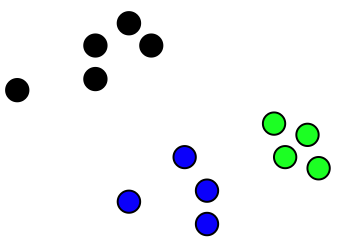
\includegraphics[height=0.25\textheight]{figures/three-class}
\end{figure}
\end{simpleblock}
\end{column}
\begin{column}{0.6\textwidth}
\onslide<3->{
\textbf{Assumption}: each class is linearly separable from the rest.\\
Ideal case: only target class has positive score.
}
\end{column}
\end{columns}

\begin{simpleblock}<2->
{Train OvA classifiers:}
\begin{figure}
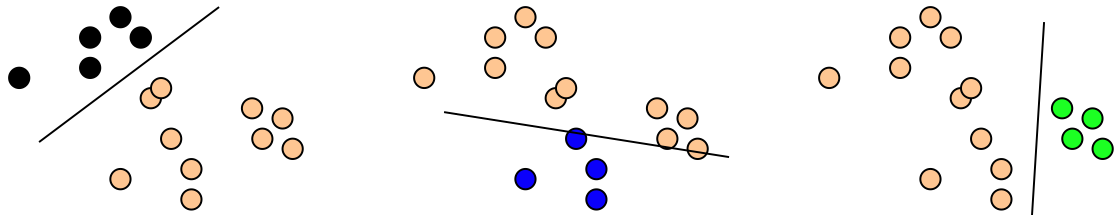
\includegraphics[height=0.25\textheight]{figures/three-class-ova}
\end{figure}
\end{simpleblock}
\note<3->{What's a failure case for OvA?}
\end{frame}

\begin{frame}
{OvA: 4-class non linearly separable example}
\begin{columns}
\begin{column}{0.4\textwidth}
Consider a dataset with four classes:
\begin{figure}
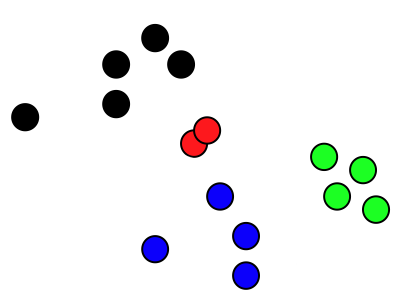
\includegraphics[height=0.25\textheight]{figures/four-class}
\end{figure}
\end{column}
\begin{column}{0.6\textwidth}
\onslide<2->{
Cannot separate \textcolor{red}{red} points from the rest.\\
Which classes might have low accuracy?
}
\note<2->[item]{Blue and green because they are getting positive score from the red classifier.}
\end{column}
\end{columns}

Train OvA classifiers:
\begin{figure}
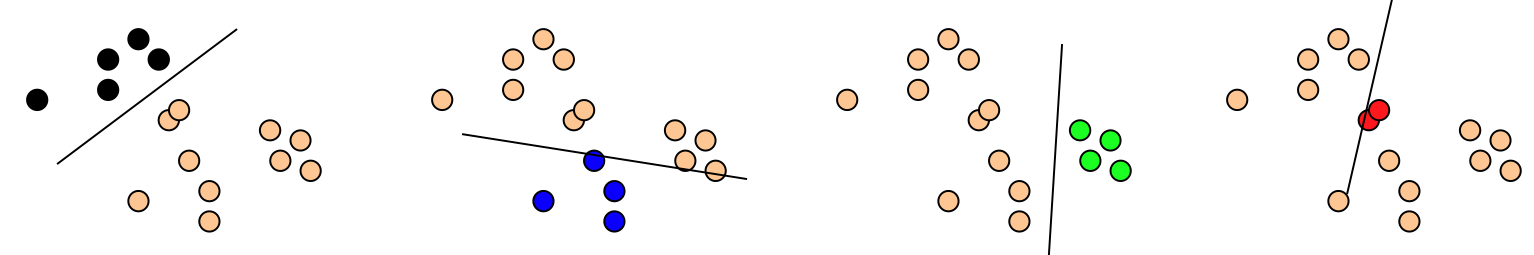
\includegraphics[height=0.25\textheight]{figures/four-class-ova}
\end{figure}
\note<2->[item]{How can we fix this? Note that optimal linear classifiers exist in this example.}
\end{frame}

\begin{frame}
{All vs All / One vs One / All pairs}
\begin{description}
    \setlength\itemsep{10pt}
\item<1->[Setting]
\begin{itemize}
    \setlength\itemsep{2pt}
\item Input space: $\cx$
\item Output space: $\cy=\left\{ 1,\ldots,k\right\} $
\end{itemize}
\note<1>[item]{How many classifiers do we need to train?}

\item<2->[Training]
\begin{itemize}
    \setlength\itemsep{2pt}
\item Train $k \choose 2$ binary classifiers, one for each pair:
$h_{ij}:\cx\to\reals$ $\text{for } i\in [1,k] \text{ and } j\in [i+1, k]$.
\item Classifier $h_{ij}$ distinguishes class $i$ (+1) from class $j$ (-1).
\end{itemize}

\item<3->[Prediction]
\begin{itemize}
    \setlength\itemsep{2pt}
\item Majority vote (each class gets $k-1$ votes)
\[
h(x)=\argmax_{i\in\left\{ 1,\ldots,k\right\} } \sum_{j\neq i}
\underbrace{h_{ij}(x)\1\pc{i<j}}_{\text{class $i$ is +1}} 
- \underbrace{h_{ji}(x)\1\pc{j<i}}_{\text{class $i$ is -1}}
\]
\note<3->[item]{Majority vote: Class $i$ gets a vote each time it is predicted.}
\item Tournament
\note<3->[item]{Tournament: start with random pairs, only winners continue.}
\item Ties can be broken arbitrarily.
\end{itemize}
\end{description}
\end{frame}

\begin{frame}
{AvA: four-class example}
\begin{columns}
\begin{column}{0.4\textwidth}
Consider a dataset with four classes:
\begin{figure}
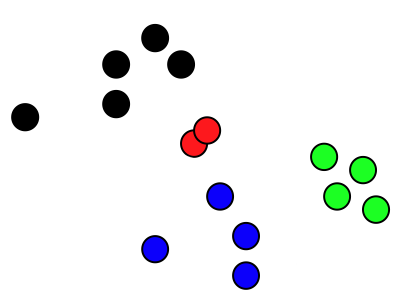
\includegraphics[height=0.25\textheight]{figures/four-class}
\end{figure}
\end{column}
\begin{column}{0.6\textwidth}
\onslide<2->{
\textbf{Assumption}: each pair of classes are linearly separable.\\
More expressive than OvA.
}
\end{column}
\end{columns}

What's the decision region for the red class?
\begin{figure}
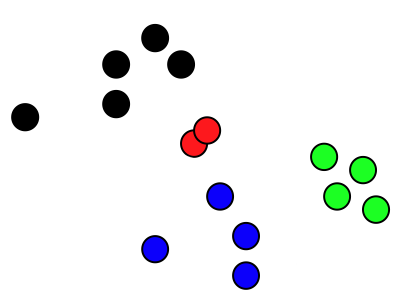
\includegraphics[height=0.3\textheight]{figures/four-class}
\end{figure}
\note<1>[item]{Draw lines separating red from each other classes. The intersection of the three regions get 3 votes (max).}
\end{frame}

\begin{frame}
{OvA vs AvA}
\begin{table}
\begin{tabular}{llcc}

\toprule
& & OvA & AvA \\
\midrule
\multirow{2}{*}{computation} & train & $O(k \onslide<2->{B_{\text{train}}(n)})$ & $O(k^2\onslide<2->{B_{\text{train}}(n/k)})$ \\
                     							   &  test & $O(k\onslide<2->{B_{\text{test}}})$ & $O(k^2 \onslide<2->{B_{\text{test}}})$ \\
       \midrule

\pause
\multirow{3}{*}{challenges}  \pause  & train & class imbalance & small training set \\
                                                   & \multirow{2}{*}{test} & \multicolumn{2}{c}{calibration / scale} \\
                                                    &         &  \multicolumn{2}{c}{tie breaking} \\
\bottomrule

\end{tabular}
\end{table}
Lack theoretical justification but simple to implement and works well in practice (when \# classes is small).

%\think{Question}: When would you prefer AvA / OvA? 
%\note{If you're using SVM, would you prefer AvA or OvA to save computation?
%Dual form would prefer AvA. When number of examples much larger than feature dimensions, dual is more expensive.}
\end{frame}

\subsection{Error correcting output codes}

\begin{frame}
{Code word for labels}
Using the reduction approach, can you train fewer than $k$ binary classifiers?
\pause

\textbf{Key idea}: Encode labels as binary codes and predict the code bits directly.
\pause

OvA encoding:
\begin{table}
\begin{tabular}{|c|c|c|c|c|}
\hline
class & $h_1$ & $h_2$ & $h_3$ & $h_4$ \\
\hline
1 & 1 & 0 & 0 & 0 \\
\hline
2 & 0 & 1 & 0 & 0\\
\hline
3 & 0 & 0 & 1 & 0\\
\hline
4 & 0 & 0 & 0 & 1\\
\hline
\end{tabular}
\end{table}
\pause

OvA uses $k$ bits to encode each label, what's the minimal number of bits you can use?
\end{frame}

\begin{frame}
{Error correcting output codes (ECOC)}
\begin{columns}
\begin{column}{0.4\textwidth}
Example: 8 classes, 6-bit code
\begin{table}
\begin{tabular}{|c|c|c|c|c|c|c|}
\hline
class & $h_1$ & $h_2$ & $h_3$ & $h_4$ &  $h_5$ & $h_6$\\
\hline
1 & 0 & 0 & 0 & 1 & 0 & 0 \\
\hline
2 & 1 & 0 & 0 & 0 & 0 & 0 \\
\hline
\rowcolor{red!20}
3 & 0 & 1 & 1 & 0 & 1 & 0\\
\hline
4 & 1 & 1 & 0 & 0 & 0 & 0 \\
\hline
5 & 1 & 1 & 0 & 0 & 1 & 0 \\
\hline
6 & 0 & 0 & 1 & 1 & 0 & 1 \\
\hline
7 & 0 & 0 & 1 & 0 & 0 & 0 \\
\hline
8 & 0 & 1 & 0 & 1 & 0 & 0 \\
\hline
\end{tabular}
\end{table}
\end{column}
%
\begin{column}{0.6\textwidth}
\begin{description}
\item<1->[Training]
Binary classifier $h_i$: 
\begin{itemize}
\item +1: classes whose $i$-th bit is 1
\item -1: classes whose $i$-th bit is 0
\end{itemize}
\item<2->[Prediction]
Closest label in terms of Hamming distance.
\begin{table}
\begin{tabular}{{|c|c|c|c|c|c|}}
\hline
$h_1$ & $h_2$ & $h_3$ & $h_4$ &  $h_5$ & $h_6$\\
\hline
0 & 1 & 1 & 0 & 1 & 1 \\
\hline
\end{tabular}
\end{table}
\item<3->[Code design]
Want good binary classifiers.
\note<3->[item]{Random or depending on domain knowledge}
\end{description}
\end{column}
\end{columns}
\end{frame}

\begin{frame}
{Error correcting output codes: summary}
\begin{itemize}
\item Computationally more efficient than OvA (a special case of ECOC). Better for large $k$.
\item Why not use the minimal number of bits ($\log_2k$)?
\pause
\begin{itemize}
\item If the minimum Hamming distance between any pair of code word is $d$, then it can correct $\left \lfloor \frac{d-1}{2} \right \rfloor$ errors.
\item In plain words, if rows are far from each other, ECOC is robust to errors.
\end{itemize}
\pause
\item Trade-off between code distance and binary classification performance.
\note<2>[item]{Larger distance -> more binary problems -> more likely to have hard binary problems.}
\item Nice theoretical results \href{http://www.jmlr.org/papers/volume1/allwein00a/allwein00a.pdf}{[Allwein et al., 2000]} (also incoporates AvA).
\end{itemize}
\end{frame}

\begin{frame}
{Review}
Reduction-based approaches:
\begin{itemize}
\item Reducing multiclass classification to binary classification: OvA, AvA%, ECOC.
\item Key is to design \textcolor{Green}{``natural'' binary classification} problems without large \textcolor{red}{computation} cost.
\end{itemize}
\pause

But,
\begin{itemize}
\item Unclear how to generalize to extremely large \# of classes.
\item ImageNet: >20k labels; Wikipedia: >1M categories.
\end{itemize}

Next,
generalize previous algorithms to multiclass settings.
\note<2->[item]{What needs to be changed? The loss function.}
\end{frame}

\section{Multiclass Loss}

\begin{frame}{Binary Logistic Regression}
\begin{itemize}
\item Given an input x, we would like to output a classification between (0,1).
\begin{align}
f(x) = sigmoid(z) = \frac{1}{1+ \exp(-z)}= \frac{1}{1 + \exp(- w^\top x-b)}.
\end{align}
\pause
\item The other class is represented in $1 - f(x)$:
\begin{align}
1 - f(x) &= \frac{\exp(-w^\top x-b)}{1 + \exp(-w^\top x-b)} = \frac{1}{1+ \exp(w^\top x +b)} = sigmoid(-z).
\end{align}
\pause
\item Another way to view: one class has $(+w, +b)$ and the other class has $(-w, -b)$.
\end{itemize}
\end{frame}

\begin{frame}{Multi-class Logistic Regression}
\begin{itemize}
  \item Now what if we have one $w_c$ for each class $c$?

  \pause
 \begin{align}
  f_c(x) = \frac{\exp(w_c^\top x) + b_c}{\sum_c \exp(w_c^\top x + b_c)}
  \end{align}
  \item Also called ``softmax'' in neural networks.

  \pause
  \item Loss function:
  $L = \sum_i -y_c^{(i)} \log f_c(x^{(i)})$

  \pause
  \item Gradient: $\frac{\partial L}{\partial z} = f - y$. Recall: MSE loss.
\end{itemize}
\end{frame}

\begin{frame}
{Comparison to OvA}
\begin{itemize}
\item \textbf{Base Hypothesis Space}: $\ch=\left\{ h:\cx\to\reals\right\} $
(\textcolor{blue}{score functions}).
\item \textbf{Multiclass Hypothesis Space} (for $k$ classes): 
\[
\cf=\left\{ x\mapsto\argmax_{i}h_{i}(x)\mid h_{1},\ldots,h_{k}\in\ch\right\} 
\]

\pause{}
\item Intuitively, $h_{i}(x)$ scores how likely $x$ is to be from class $i$.

\item OvA objective: $h_i(x) > 0$ for $x$ with label $i$ and
$h_i(x) < 0$ for $x$ with all other labels.

\pause
\item At test time, to predict $(x, i)$ correctly we only need
\begin{align}
h_i(x) > h_j(x) \qquad \forall j \neq i .
\end{align}
\end{itemize}
\end{frame}

\begin{frame}
{Multiclass Perceptron}
\begin{itemize}
\item Base linear predictors: $h_i(x) = w_i^Tx$ ($w\in \bR^d$).
\pause
\item Multiclass perceptron:
\begin{algorithm}[H]
	Given a multiclass dataset $\sD=\pc{(x, y)}$\;
	Initialize $w\leftarrow 0$\;
	\For{$\text{iter} = 1,2,\ldots,T$}{
	\For{$(x,y) \in \sD$}
 	{
 		$\hat{y} = \argmax_{y'\in\sY} w_{y'}^Tx$\;
 		\If(\tcp*[h]{We've made a mistake}){$\hat{y} \neq y$}{ 
 		$w_y \leftarrow w_y + x$ \tcp*[l]{Move the target-class scorer towards $x$}
 		$w_{\hat{y}} \leftarrow w_{\hat{y}} - x$ \tcp*[l]{Move the wrong-class scorer away from $x$}
 		}
  	}
  	}
\end{algorithm}
\end{itemize}
\end{frame}

% \begin{frame}{Linear Binary Classifier Review}

% \begin{itemize}
% \item Input Space: $\cx=\reals^{d}$
% \item Output Space: $\cy=\left\{ -1,1\right\} $ 
% \end{itemize}

% \begin{itemize}
% \item Linear classifier score function:
% \begin{eqnarray*}
% f(x) & = & \left\langle w,x\right\rangle =w^{T}x
% \end{eqnarray*}

% \pause{}
% \item Final classification prediction: $\sign\left(f(x)\right)$
% \item Geometrically, when are $\sign\left(f(x)\right)=+1$ and $\sign\left(f(x)\right)=-1$? 
% \end{itemize}
% \end{frame}
% %
% \begin{frame}{Linear Binary Classifier Review}

% \begin{center}
% 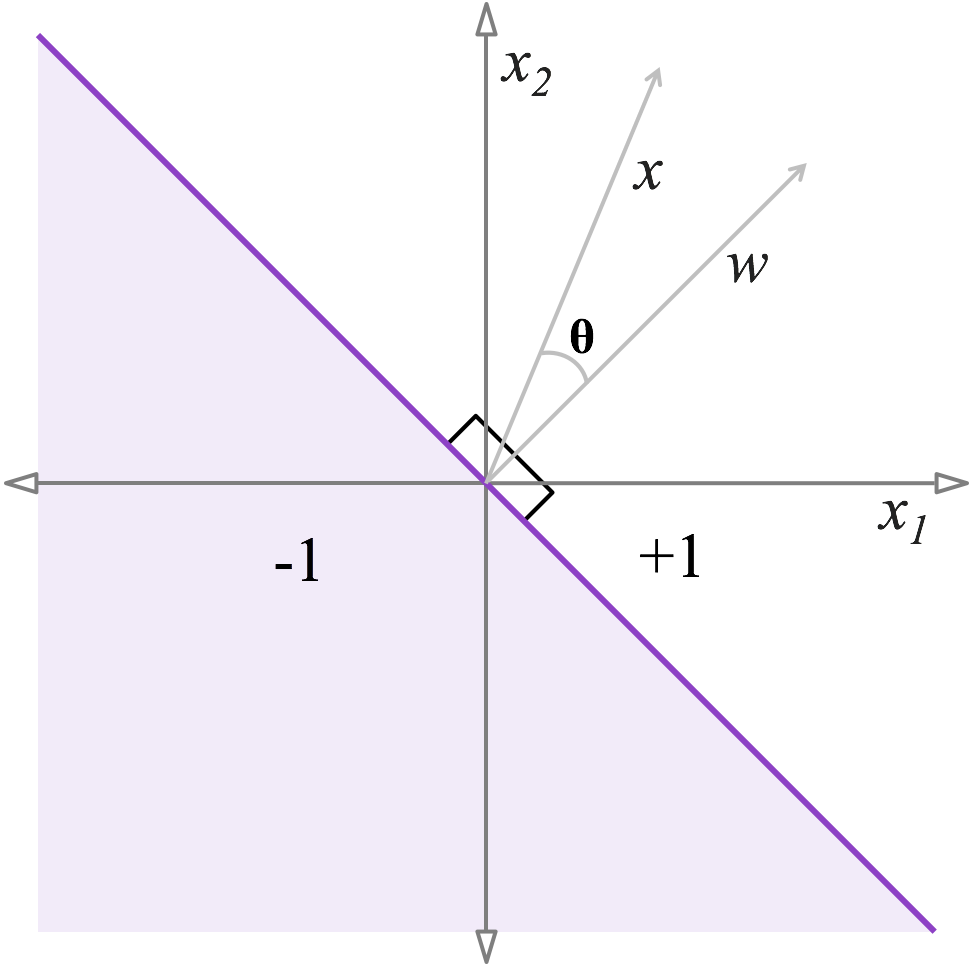
\includegraphics[height=0.45\textheight]{figures/linear-separator}
% \par\end{center}

% Suppose $\|w\|>0$ and $\|x\|>0$: 
% \begin{eqnarray*}
% f(x) & = & \left\langle w,x\right\rangle =\|w\|\|x\|\cos\theta\\
% f(x)>0 & \iff & \cos\theta>0 \iff\theta\in\left(-90^{\circ},90^{\circ}\right)\\
% f(x)<0 & \iff & \cos\theta<0 \iff\theta\not\in[-90^{\circ},90^{\circ}]
% \end{eqnarray*}

% \end{frame}

\begin{frame}
{Rewrite the scoring function}
\begin{itemize}
\item Remember that we want to scale to very large \# of classes and
reuse algorithms and analysis for binary classification
\begin{itemize}
\item $\implies$ a \textcolor{blue}{single weight vector} is desired
\end{itemize}

\item How to rewrite the equation such that we have one $w$ instead of $k$?
\pause
\begin{align}
w_i^Tx &= w^T\psi(x, i) \\
h_i(x) &= h(x, i)
\end{align}
\begin{itemize}
\item Encode labels in the feature space.
\item Score for each label $\rightarrow$ score for the ``\emph{compatibility}'' of a label and an input.
\end{itemize}
\end{itemize}
\end{frame}

\begin{frame}{The Multivector Construction}
How to construct the feature map $\psi$?
\pause
\begin{itemize}
\item What if we stack $w_{i}$'s together (\eg $x\in \bR^2, \sY = \pc{1,2,3}$)
\[
w=\left(\underbrace{-\frac{\sqrt{2}}{2},\frac{\sqrt{2}}{2}}_{w_{1}},\underbrace{0,1}_{w_{2}},\underbrace{\frac{\sqrt{2}}{2},\frac{\sqrt{2}}{2}}_{w_{3}}\right)
\]
\end{itemize}
\pause
\begin{itemize}
\item And then do the following: $\Psi:\reals^{2}\times\left\{ 1,2,3\right\} \to\reals^{6}$
defined by
\begin{eqnarray*}
\Psi(x,1) & := & \left(x_{1},x_{2},0,0,0,0\right)\\
\Psi(x,2) & := & \left(0,0,x_{1},x_{2},0,0\right)\\
\Psi(x,3) & := & \left(0,0,0,0,x_{1},x_{2}\right)
\end{eqnarray*}
\pause
\item Then $\left\langle w,\Psi(x,y)\right\rangle =\left\langle w_{y},x\right\rangle $,
which is what we want. 
\end{itemize}
\end{frame}


\begin{frame}
{Rewrite multiclass perceptron}
Multiclass perceptron using the multivector construction.

\begin{algorithm}[H]
	Given a multiclass dataset $\sD=\pc{(x, y)}$\;
	Initialize $w\leftarrow 0$\;
	\For{$\text{iter} = 1,2,\ldots,T$}{
	\For{$(x,y) \in \sD$}
 	{
 		$\hat{y} = \argmax_{y'\in \sY} w^T\psi(x, y')$ \tcp*[l]{Equivalent to $\argmax_{y'\in\sY} w_{y'}^Tx$}
 		\If(\tcp*[h]{We've made a mistake}){$\hat{y} \neq y$}{ 
 		$w \leftarrow w + \psi(x, y)$ \tcp*[l]{Move the scorer towards $\psi(x, y)$}
 		$w \leftarrow w - \psi(x, \hat{y})$ \tcp*[l]{Move the scorer away from $\psi(x, \hat{y})$}
 		}
  	}
  	}
\end{algorithm}
\pause
\textcolor{Green}{Exercise}: What is the base binary classification problem in multiclass perceptron?
\note{$w^T(\phi(x,i)-\phi(x,j)) > 0$.}
\end{frame}

\begin{frame}
{Features}
Toy multiclass example: Part-of-speech classification
\begin{itemize}
\item $\cx=\left\{ \mbox{All possible words}\right\} $
\item $\cy=\left\{ \mbox{NOUN,VERB,ADJECTIVE,\ldots}\right\} $.
\note<1>{What are useful features?}
\pause{}
\item Features of $x\in\cx$: $\mbox{[The word itself], ENDS\_IN\_ly, ENDS\_IN\_ness, ...}$
\end{itemize}

How to construct the feature vector?
\begin{itemize}
\item Multivector construction: $w\in \bR^{d\times k}$---\textcolor{red}{doesn't scale}.
\pause
\item Directly design features for each class.
\begin{align}
\Psi(x,y)=\left(\psi_{1}(x,y),\psi_{2}(x,y),\psi_{3}(x,y),\ldots,\psi_{d}(x,y)\right)
\end{align}
\begin{itemize}
\item Size can be bounded by $d$.
\end{itemize}
\end{itemize}
\end{frame}

\begin{frame}
{Features}
Sample training data:
\begin{center}
\texttt{
The boy grabbed the apple and ran away quickly .
}
\end{center}
\pause

Feature:
\begin{eqnarray*}
\psi_{1}(x,y) & = & \ind{x=\mbox{apple AND }y=\mbox{NOUN}}\\
\psi_{2}(x,y) & = & \ind{x=\mbox{run AND }y=\mbox{NOUN}}\\
\psi_{3}(x,y) & = & \ind{x=\mbox{run AND }y=\mbox{VERB}}\\
\psi_{4}(x,y) & = & \ind{x\mbox{ ENDS\_IN\_ly AND \ensuremath{y=}ADVERB}}\\
\ldots
\end{eqnarray*}
\pause
\vspace{-2em}
\begin{itemize}[<+->]
\item E.g., $\Psi(x=\text{run},y=\text{NOUN})=\left(0,1,0,0,\ldots\right)$
\item After training, what's $w_{1},w_{2},w_{3},w_{4}$?
\item \textcolor{blue}{No need to include features unseen in training data}.
\end{itemize}

\end{frame}

\begin{frame}
{Feature templates: implementation}
\begin{itemize}
\item Flexible, \eg neighboring words, suffix/prefix.
\item ``Read off'' features from the training data.
\item Often sparse---efficient in practice, \eg NLP problems.
\item Can use a hash function: template $\rightarrow \pc{1, 2, \ldots, d}$.
\end{itemize}
\end{frame}

\begin{frame}
{Review}
Ingredients in multiclass classification:
\begin{itemize}
\item Scoring functions for each class (similar to ranking).
\item Represent labels in the input space $\implies$ single weight vector.
\end{itemize}
\pause

We've seen
\begin{itemize}
\item How to generalize the perceptron algorithm to multiclass setting.
\item Very simple idea. Was popular in NLP for structured prediction (\eg tagging, parsing).
\end{itemize}
\pause

Next,
\begin{itemize}
\item How to generalize SVM to the multiclass setting.
\item \think{Concept check}: Why might one prefer SVM / perceptron?
\note{Uniqueness of solution, online learning / efficiency, inductive bias (margin)}
\end{itemize}
\end{frame}

%================================== 


\subsection{Linear Multiclass SVM}
\subsubsection{Formulation through constraints on margin}

\begin{frame}{Margin for Multiclass}
\begin{description}
\item<1->[Binary]
\begin{itemize}
\item Margin for $(\xn, \yn)$:
\begin{align}
\yn w^T\xn
\end{align}
\item Want margin to be large and positive ($w^T\xn$ has same sign as $\yn$)
\end{itemize}

\item<2->[Multiclass]
\begin{itemize}
\item Class-specific margin for $(\xn, \yn)$:
\begin{align}
h(\xn,\yn)-h(\xn,y).
\end{align}
\item Difference between scores of the correct class and each other class
\item Want margin to be large and positive for all $y\neq \yn$. 
\end{itemize}
\end{description}
\end{frame}
%

\begin{frame}
{Multiclass SVM: separable case}
\begin{description}
\item<1->[Binary] 
\begin{align}
\min_w \quad & \frac{1}{2}\|w\|^2 \\
\text{s.t.} \quad& \underbrace{\yn w^T\xn}_{\text{margin}} \geq 1 \quad \forall (\xn, \yn) \in \sD
\end{align}

\item<2->[Multiclass] As in the binary case, take 1 as our target margin.
\begin{align}
m_{n,y}(w)&\eqdef \underbrace{\left\langle w,\Psi(\xn,\yn)\right\rangle}_{\text{score of correct class}}
- \underbrace{\left\langle w,\Psi(\xn,y)\right\rangle}_{\text{score of other class}} \\
\min_w \quad & \frac{1}{2}\|w\|^2 \\
\text{s.t.} \quad& m_{n,y}(w) \geq 1 \quad
\forall (\xn, \yn) \in \sD,\, y\neq \yn
\end{align}

\end{description}
\onslide<3->{
\think{Exercise}: write the objective for the non-separable case
}
\note<3->{Next, let's think about how to write the objective using hinge loss.}
\end{frame}

\subsubsection{Formulation through hinge loss}
\begin{frame}
{Recap: hingle loss for binary classification}
\begin{itemize}
\item Hinge loss: a convex upperbound on the 0-1 loss
\begin{align}
\ell_{\text{hinge}}(y, \hat{y}) = \max(0, 1 -  yh(x))
\end{align}
\begin{figure}
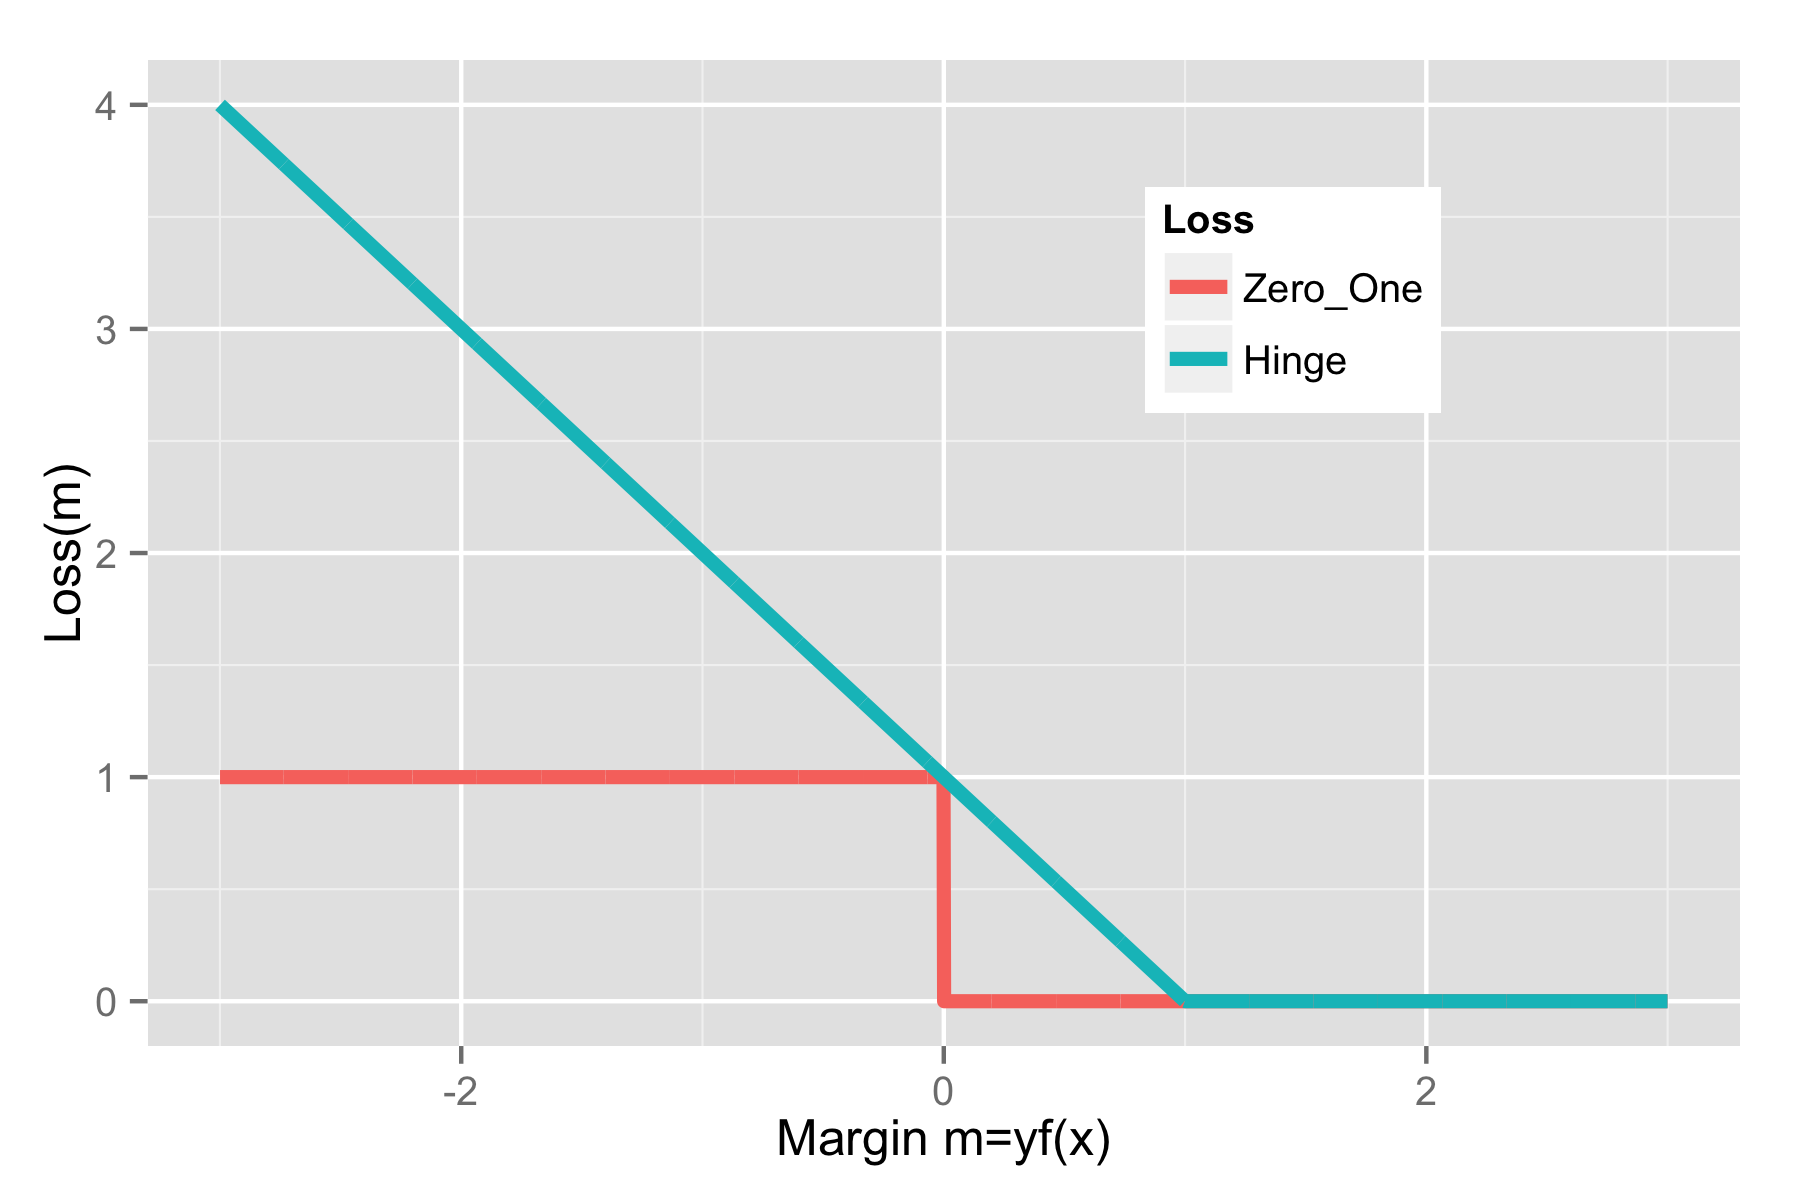
\includegraphics[height=0.5\textheight]{{figures/loss.Zero_One.Hinge}.png}
\end{figure}
\end{itemize}
\end{frame}

\begin{frame}
{Generalized hinge loss}
\begin{itemize}[<+->]
\item What's the zero-one loss for multiclass classification?
\begin{align}
\onslide<+->{\Delta(y, y') = \1\pc{y\neq y'}}
\end{align}
\item In general, can also have different cost for each class.

\item Upper bound on $\Delta(y, y')$.
\begin{align}
\hat{y} &\eqdef \argmax_{y'\in\sY} \left\langle w, \Psi(x, y') \right\rangle \\
\onslide<+->{
\implies & \left\langle w, \Psi(x, y) \right\rangle \leq
\left\langle w, \Psi(x, \hat{y}) \right\rangle \\
}
\onslide<+->{
\implies & \Delta(y, \hat{y}) \leq \Delta(y, \hat{y}) -
\left\langle w, \p{\Psi(x, {y}) - \Psi(x, \hat{y}}) \right\rangle
&& \text{When are they equal?}
}
\end{align}

\item Generalized hinge loss:
\begin{align}
\ell_\text{hinge}(y, x, w) \eqdef
\max_{y'\in\sY}\p{
\Delta(y, {y'}) -
\left\langle w, \p{\Psi(x, {y}) - \Psi(x, {y'}}) \right\rangle
}
\end{align}
% \note<+->{When $y'=y$, $\ell_{\text{hinge}}=0$.}
\end{itemize}
\end{frame}

\begin{frame}{Multiclass SVM with Hinge Loss}
 
\begin{itemize}
\item Recall the hinge loss formulation for binary SVM (without the bias term):
\[
\min_{w\in\reals^{d}}\frac{1}{2}||w||^{2}+C\sum_{n=1}^{N}\max\left(0,1-\underbrace{\yn w^{T}\xn}_{\text{margin}}\right).
\]

\pause{}
\item The multiclass objective: 
\[
\min_{w\in\reals^{d}}\frac{1}{2}||w||^{2}+
C\sum_{n=1}^{N}\max_{y'\in\sY} \p{
\Delta(y, {y'}) -
\underbrace{
\left\langle w, \p{\Psi(x, {y}) - \Psi(x, {y'}}) \right\rangle
}_{\text{margin}}
}
\]

\begin{itemize}
\item $\Delta(y, y')$ as \textcolor{blue}{target margin} for each class.
\item If margin $m_{n, y'}(w)$ meets or exceeds its target $\Delta(\yn,y')$
$\forall y\in \sY$, then no loss on example $n$. 
\note<2->{If exceeds margin, loss is negative, which must be smaller than loss of the true class, which is zero.}
\end{itemize}
\end{itemize}
\end{frame}
%

\subsection{Is This Worth The Hassle Compared to One-vs-All?}
\begin{frame}{Recap: What Have We Got?}
\begin{itemize}
\item Problem: Multiclass classification $\cy=\left\{ 1,\ldots,k\right\} $
\end{itemize}

\pause{}
\begin{itemize}
\item Solution 1: One-vs-All


\begin{itemize}
\item Train $k$ models: $h_{1}(x),\ldots,h_{k}(x):\cx\to\reals$.


\item Predict with $\argmax_{y\in\cy}h_{y}(x)$.


\item Gave simple example where this fails for linear classifiers
\end{itemize}
\end{itemize}

\pause{}
\begin{itemize}
\item Solution 2: Multiclass loss


\begin{itemize}
\item Train one model: $h(x,y):\cx\times\cy\to\reals$.


\item Prediction involves solving $\argmax_{y\in\cy}h(x,y)$.
\end{itemize}
\end{itemize}
\end{frame}
%
\begin{frame}{Does it work better in practice?}
\begin{itemize}
\item Paper by Rifkin \& Klautau: ``\href{http://www.jmlr.org/papers/v5/rifkin04a.html}{In Defense of One-Vs-All Classification}''
(2004)
\begin{itemize}
\item Extensive experiments, carefully done 
\begin{itemize}
\item albeit on relatively small UCI datasets
\end{itemize}
\end{itemize}


\begin{itemize}
\item Suggests one-vs-all works just as well in practice
\begin{itemize}
\item (or at least, the advantages claimed by earlier papers for multiclass
methods were not compelling)
\end{itemize}
\end{itemize}
\end{itemize}

\pause
\begin{itemize}
\item Compared 
\begin{itemize}
\item many multiclass frameworks (including the one we discuss)
\item one-vs-all for SVMs with RBF kernel
\item one-vs-all for square loss with RBF kernel (for classification!) 
\end{itemize}
\end{itemize}


\begin{itemize}
\item All performed roughly the same
\end{itemize}
\end{frame}
%
\begin{frame}{Why Are We Bothering with Multiclass?}
\begin{itemize}
\item The framework we have developed for multiclass
\begin{itemize}
\item compatibility features / scoring functions
\item multiclass margin
\item target margin / multiclass loss
\end{itemize}
\end{itemize}

\pause{}
\begin{itemize}
\item Generalizes to situations where \textcolor{blue}{$k$ is very large} and one-vs-all
is intractable.
\end{itemize}

\pause{}
\begin{itemize}
\item Key idea is that we can \textcolor{blue}{generalize across outputs $y$ by using features
of $y$}.
\end{itemize}
\end{frame}

\section{Introduction to Structured Prediction}
\begin{frame}{Example: Part-of-speech (POS) Tagging}

\begin{itemize}
\item Given a sentence, give a part of speech tag for each word:
\end{itemize}
\begin{center}
\begin{tabular}{|c|c|c|c|c|}
\hline 
$x$ & $\underbrace{\mbox{[START]}}_{x_{0}}$ & $\underbrace{\mbox{He}}_{x_{1}}$ & $\underbrace{\mbox{eats}}_{x_{2}}$ & $\underbrace{\mbox{apples}}_{x_{3}}$\tabularnewline
\hline 
$y$ & $\underbrace{\mbox{[START]}}_{y_{0}}$ & $\underbrace{\mbox{Pronoun}}_{y_{1}}$ & $\underbrace{\mbox{Verb}}_{y_{2}}$ & $\underbrace{\mbox{Noun}}_{y_{3}}$\tabularnewline
\hline 
\end{tabular}
\par\end{center}

\pause{}
\begin{itemize}
\item $\cv=\left\{ \mbox{all English words}\right\} \cup\left\{ \mbox{[START]},"."\right\} $
\item $\cx=\cv^{n}$, $n=1,2,3,\ldots$ {[}Word sequences of any length{]}

\pause{}
\item $\cp=\left\{ \mbox{START},\mbox{Pronoun,Verb,Noun,Adjective}\right\} $
\item $\cy=\cp^{n},\,n=1,2,3,\ldots${[}Part of speech sequence of any length{]}

\end{itemize}
\end{frame}

\begin{frame}{Multiclass Hypothesis Space}

\begin{itemize}
\item \textcolor{blue}{Discrete} output space: $\cy(x)$ 
\begin{itemize}
\item Very large but has structure, e.g., linear chain (sequence labeling), tree (parsing)
\item Size depends on input $x$
\end{itemize}

\pause{}
\item Base Hypothesis Space: $\ch=\left\{ h:\cx\times\cy\to\reals\right\} $
\begin{itemize}
\item $h(x,y)$ gives \textcolor{blue}{compatibility score} between input $x$ and
output $y$ 
\end{itemize}

\pause{}
\item Multiclass hypothesis space
\[
\cf=\left\{ x\mapsto\argmax_{y\in\cy}h(x,y)\mid h\in\ch\right\} 
\]


\item Final prediction function is an $f\in\cf$. 
\item For each $f\in\cf$ there is an underlying compatibility score function
$h\in\ch$. 
\end{itemize}
\end{frame}
%

\begin{frame}{Structured Prediction}
\begin{itemize}
\item Part-of-speech tagging
\begin{table}
\begin{tabular}{llll}
$x\colon$ & he & eats & apples \\
$y\colon$ & pronoun & verb & noun 
\end{tabular}
\end{table}

\item Multiclass hypothesis space:
\begin{align}
& h(x,y) = w^T \Psi(x, y) \\
& \cf = \left\{ x\mapsto\argmax_{y\in\cy}h(x,y)\mid h\in\ch\right\}
\end{align}
\end{itemize}

\begin{itemize}
\item A special case of multiclass classification
\item  How to design the feature map $\Psi$? What are the considerations?
\note{contextual dependence, efficient argmax}
\end{itemize}
\end{frame}
%
\begin{frame}{Unary features}

\begin{itemize}
\item A  \textbf{unary feature} only depends on 
\begin{itemize}
\item the label at a \textcolor{blue}{single position}, $y_{i}$, and $x$ 
\end{itemize}

\item Example: 
\begin{eqnarray*}
\phi_{1}(x,y_{i}) & = & \ind{x_{i}=\mbox{runs}}\ind{y_{i}=\mbox{Verb}}\\
\phi_{2}(x,y_{i}) & = & \ind{x_{i}=\mbox{runs}}\ind{y_{i}=\mbox{Noun}}\\
\phi_{3}(x,y_{i}) & = & \ind{x_{i-1}=\mbox{He}}\ind{x_{i}=\mbox{runs}}\ind{y_{i}=\mbox{Verb}}
\end{eqnarray*}
 
\end{itemize}
\end{frame}
%
\begin{frame}{Markov features}

\begin{itemize}
\item A \textbf{markov feature} only depends on 
\begin{itemize}
\item two \textcolor{blue}{adjacent} labels, $y_{i-1}$ and $y_{i}$,
and $x$
\end{itemize}

\item Example: 
\begin{eqnarray*}
\theta_{1}(x,y_{i-1},y_{i}) & = & \ind{y_{i-1}=\mbox{Pronoun}}\ind{y_{i}=\mbox{Verb}}\\
\theta_{2}(x,y_{i-1},y_{i}) & = & \ind{y_{i-1}=\mbox{Pronoun}}\ind{y_{i}=\mbox{Noun}}
\end{eqnarray*}

\item Reminiscent of Markov models in the output space
\item Possible to have higher-order features 
 
\end{itemize}
\end{frame}
%
\begin{frame}{Local Feature Vector and Compatibility Score}
\begin{itemize}[<+->]
\item At each position $i$ in sequence, define the \textbf{local feature
vector} (\textcolor{blue}{unary} and \textcolor{red}{markov}):
\begin{eqnarray*}
\Psi_{i}(x,y_{i-1},y_{i}) & = & (\phi_{1}(x,{\color{blue}y_{i}}),\phi_{2}(x,{\color{blue}y_{i}}),\ldots,\\
 &  & \theta_{1}(x,{\color{red}y_{i-1},y_{i}}),\theta_{2}(x,{\color{red}y_{i-1},y_{i}}),\ldots)
\end{eqnarray*}

\item And \textbf{local compatibility score} at position $i$:
$\left\langle w,\Psi_{i}(x,y_{i-1},y_{i})\right\rangle $. 

\item The compatibility score for $\left(x,y\right)$
is the sum of local compatibility scores: 
\begin{align}
\sum_{i}\left\langle w,\Psi_{i}(x,y_{i-1},y_{i})\right\rangle 
= \left\langle w,\sum_{i}\Psi_{i}(x,y_{i-1},y_{i})\right\rangle
= \left\langle w,\Psi(x,y)\right\rangle ,
\end{align}
where we define the \textbf{sequence feature vector} by 
\[
\Psi(x,y)=\sum_{i}\Psi_{i}(x,y_{i-1},y_{i}). \qquad \text{\color{blue}decomposable}
\]
\end{itemize}
\end{frame}

\begin{frame}
{Structured perceptron}
\begin{algorithm}[H]
	Given a dataset $\sD=\pc{(x, y)}$\;
	Initialize $w\leftarrow 0$\;
	\For{$\text{iter} = 1,2,\ldots,T$}
	{
	\For{$(x,y) \in \sD$}
 	{
 		$\hat{y} = \argmax_{y'\in{\color<2->{red}\sY(x)}} w^T\psi(x, y')$\;
 		\If(\tcp*[h]{We've made a mistake}){$\hat{y} \neq y$}{ 
 		$w \leftarrow w + \Psi(x, y)$ \tcp*[l]{Move the scorer towards $\psi(x, y)$}
 		$w \leftarrow w - \Psi(x, \hat{y})$ \tcp*[l]{Move the scorer away from $\psi(x, \hat{y})$}
 		}
  	}
  	}
\end{algorithm}
\onslide<2->{
Identical to the multiclass perceptron algorithm except the $\argmax$ is now over the structured output space $\sY(x)$.
}
\end{frame}
%

\begin{frame}
{Structured hinge loss}
\begin{itemize}
\item Recall the generalized hinge loss
\begin{align}
\ell_\text{hinge}(y, \hat{y}) \eqdef
\max_{y'\in{\color{blue}\sY(x)}}\p{
\Delta(y, {y'}) +
\left\langle w, \p{\Psi(x, {y'}) - \Psi(x, {y}}) \right\rangle
}
\end{align}

\item What is $\Delta(y, {y'})$ for two sequences?
\pause
\item \textbf{Hamming loss} is common:
\[
\Delta(y,y')=\frac{1}{L}\sum_{i=1}^{L}\ind{y_{i}\neq y_{i}'}
\]
where $L$ is the sequence length.

%\item Can generalize to the cost-sensitive version using $\delta(y_{i},y_{i}')$

\end{itemize}
\end{frame}

\begin{frame}
{Structured SVM}
\textcolor{Green}{Exercise}:
\begin{itemize}
\item Write down the objective of structured SVM using the structured hinge loss.

\item Stochastic sub-gradient descent for structured SVM (similar to HW3 P3)
\item Compare with the structured perceptron algorithm
\end{itemize}
\end{frame}

\begin{frame}
{The argmax problem for sequences}
% \pause
\begin{description}[<+->]
\item[Problem]
To compute predictions, we need to find 
$\argmax_{y\in\cy(x)}\left\langle w,\Psi(x,y)\right\rangle$, and $\left|\cy(x)\right|$ is \textcolor{blue}{exponentially} large.

\item[Observation]
$\Psi(x,y)$ decomposes to $\sum_i \Psi_i(x,y)$.

\item[Solution]
Dynamic programming (similar to the Viterbi algorithm)
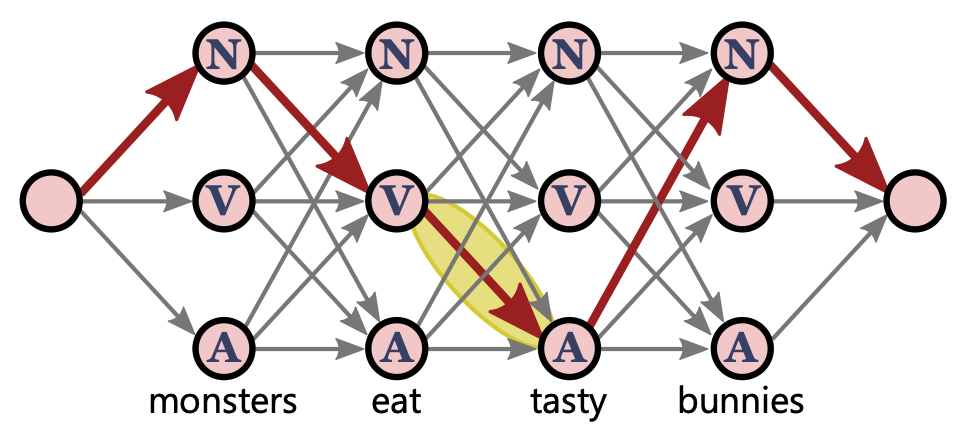
\includegraphics[height=0.4\textheight]{figures/dp}
What's the running time?
\note<.>{Let $K=\vert\sY\vert$, DP runtime $O(K^2L)$, $m$th order Markov feature has runtime $O(K^mL)$, naive runtime $O(K^L)$.}
\end{description}
\let\thefootnote\relax\footnotetext{\tiny{Figure by Daum\'e III. A course in machine learning. Figure 17.1}.}
\end{frame}

% \begin{frame}
% {The argmax problem in general}
% Efficient problem-specific algorithms:
% \begin{table}
% \begin{tabular}{llll}
% \toprule
% problem & structure & algorithm \\
% \midrule
% constituent parsing & binary trees with context-free features & CYK  \\
% dependency parsing & spanning trees with edge features & Chu-Liu-Edmonds \\
% image segmentation & 2d with adjacent-pixel features & graph cuts \\
% \bottomrule
% \end{tabular}
% \end{table}
% \pause

% General algorithm:
% \begin{itemize}
% \item Integer linear programming (ILP)
% \begin{align}
% \max_z\; a^Tz \quad \text{s.t. linear constraints on $z$}
% \end{align}
% \item $z$: indicator of substructures, \eg $\1\pc{y_i=\text{article and }y_{i+1}=\text{noun}}$
% \item constraints: $z$ must correspond to a valid structure
% \end{itemize}
% \end{frame}

% Additional resource:
% https://people.cs.umass.edu/~mccallum/papers/crf-tutorial.pdf
\begin{frame}{Conditional random field (CRF)}
\begin{itemize}
\item Recall that we can write logistic regression in a general form:
\[
p(y|x) = \frac{1}{Z(x)} \exp(w^\top \psi(x, y)).
\]
\item $Z$ is normalization constant: $Z(x) = \sum_{y \in Y} \exp(w^\top \psi(x, y))$.
\pause
\item Example: linear chain $\{y_t\}$
\item We can incorporate unary and Markov features:
$p(y|x) = \frac{1}{Z(x)} \exp(\sum_t w^\top \psi(x, y_t, y_{t-1}))$
\begin{center}
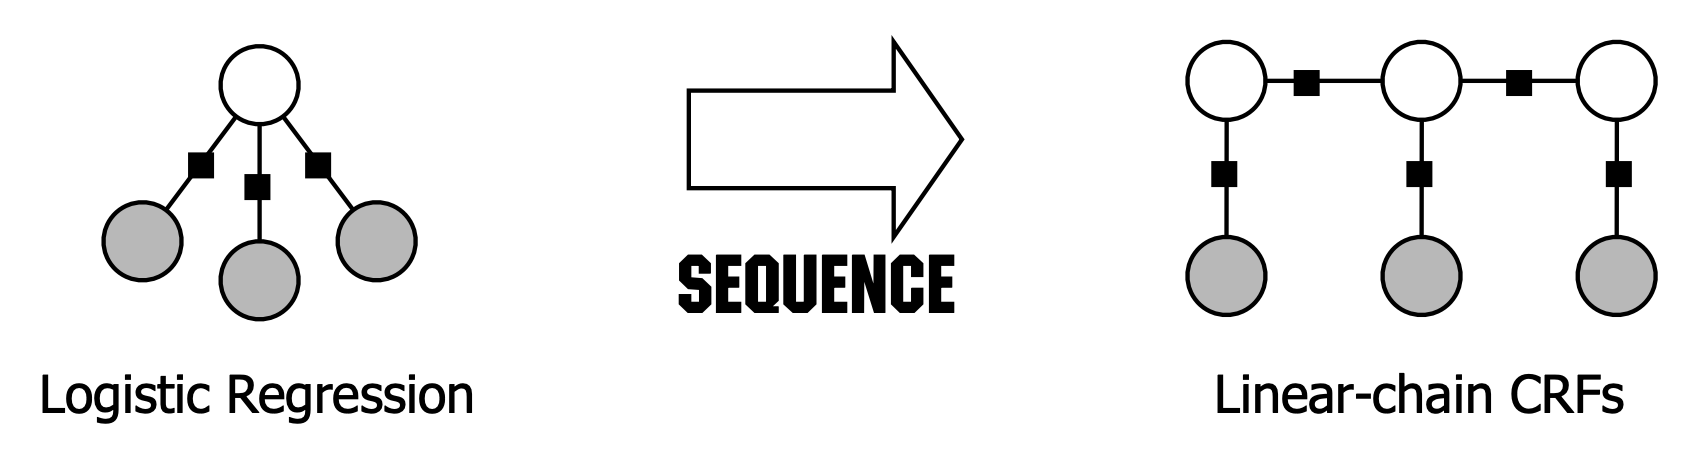
\includegraphics[width=0.6\textwidth]{figures/crf.png}
\end{center}
% \item Unary energy
% \item Pairwise energy
% \item Total energy
\end{itemize}
\end{frame}

\begin{frame}{Conditional random field (CRF)}
\begin{itemize}
  \item Compared to Structured SVM, CRF has a probabilistic interpretation.
  \item We can draw samples in the output space.
  \pause
  \item How do we learn $w$? Maximum log likelihood, and regularization term: $\lambda \lVert w \rVert^2$
  \item Loss function:
  \begin{align*}
  l(w) &= - \frac{1}{N} \sum_{i=1}^{N} \log p(y^{(i)} | x^{(i)}) + \frac{1}{2} \lambda \lVert w \rVert^2 \\
  &= - \frac{1}{N} \sum_i \sum_t \sum_k w_k \psi_k(y^{(i)}_t, y^{(i)}_{t-1}) + \frac{1}{N} \sum_{i} \log Z(x^{(i)}) + \frac{1}{2}  \sum_k \lambda w_k^2
  \end{align*}
\end{itemize}
\end{frame}

\begin{frame}{Conditional random field (CRF)}
\begin{itemize}
  \item Loss function:
  \[
  l(w)= - \frac{1}{N} \sum_i \sum_t \sum_k w_k \psi_k(x^{(i)}, y^{(i)}_t, y^{(i)}_{t-1}) + \frac{1}{N} \sum_{i} \log Z(x^{(i)}) +\frac{1}{2} \sum_k  \lambda w_k^2
  \]
\item Gradient:
\begin{align}
\frac{\partial l(w)}{\partial w_k} &= -\frac{1}{N} \sum_i \sum_t \sum_k \psi_k(x^{(i)}, y^{(i)}_t, y^{(i)}_{t-1}) \\
& + \frac{1}{N} \sum_{i} \frac{\partial}{\partial w_k} \log \sum_{y' \in Y} \exp(\sum_t \sum_{k'} w_{k'} \psi_{k'}(x^{(i)}, y'_t, y'_{t-1})) + \sum_k \lambda w_k
\end{align}
\end{itemize}
\end{frame}

\begin{frame}{Conditional random field (CRF)}
\begin{itemize}
  \item What is $\frac{1}{N} \sum_i \sum_t \sum_k \psi_k(x^{(i)}, y^{(i)}_t, y^{(i)}_{t-1})$?
  \pause

  \item It is the expectation $\psi_k (x^{(i)}, y_t, y_{t-1})$ under the empirical distribution $\tilde{p}(x, y) = \frac{1}{N} \sum_i \mathbbm{1} [x = x^{(i)}] \mathbbm{1} [y = y^{(i)}]$.
\end{itemize}
\end{frame}


\begin{frame}{Conditional random field (CRF)}
\begin{itemize}
  \item What is $\frac{1}{N} \sum_i \frac{\partial}{\partial w_k} \log \sum_{y' \in Y} \exp(\sum_t \sum_{k'} w_{k'} \psi_{k'}(x^{(i)}, y_t', y_{t-1}'))$?
  \pause
  \begin{align}
  & \frac{1}{N} \sum_i \frac{\partial}{\partial w_k} \log \sum_{y' \in Y} \exp(\sum_t \sum_{k'} w_{k'} \psi_{k'}(x^{(i)}, y_t', y_{t-1}'))\\
  &= \frac{1}{N} \sum_i \left[\sum_{y' \in Y} \exp(\sum_t \sum_{k'} w_{k'} \psi_{k'}(x^{(i)}, y_t', y_{t-1}'))\right]^{-1}\\
  &\left[\sum_{y' \in Y} \exp(\sum_t \sum_{k'} w_{k'} \psi_{k'}(x^{(i)}, y_t^{(i)}, y_{t-1}^{(i)})) \sum_t \psi_k(x^{(i)}, y_t', y_{t-1}') \right] \\
  &= \frac{1}{N} \sum_i \sum_t \sum_{y'\in Y} p(y'_t, y_{t-1}' | x) \psi_k (x^{(i)}, y'_t, y'_{t-1})
  \end{align}
  \pause
  \item It is the expectation of $\psi_k (x^{(i)}, y'_t, y'_{t-1})$ under the model distribution $p(y'_t, y_{t-1}' | x)$.
\end{itemize}
\end{frame}

\begin{frame}{Conditional random field (CRF)}
\begin{itemize}
  \item To compute the gradient, we need to infer expectation under the model distribution $p(y|x)$.
  \pause
  \item Compare the learning algorithms: in structured SVM we need to compute the argmax, whereas in CRF we need to compute the model expectation.
  \pause
  \item Both problems are NP-hard for general graphs.
\end{itemize}
\end{frame}

\begin{frame}{CRF Inference}
\begin{itemize}
  \item In the linear chain structure, we can use the forward-backward algorithm for inference, similar to Viterbi.
  \pause
  \item Initiate $\alpha_j(1) = \exp (w^\top \psi(y_1=j, x_1))$
  \pause
  \item Recursion: $\alpha_j(t) = \sum_i \alpha_i (t-1) \exp(w^\top \psi(y_t=j, y_{t-1}=i, x_t))$
  \pause
  \item Result: $Z(x) = \sum_j \alpha_j(T)$
  \pause
  \item Similar for the backward direction.
  \pause
  \item Test time, again use Viterbi algorithm to infer argmax.
  \pause
  \item The inference algorithm can be generalized to belief propagation (BP) in a tree structure (exact inference).
  \pause
  \item In general graphs, we rely on approximate inference (e.g. loopy belief propagation).
\end{itemize}
\end{frame}

\begin{frame}{Examples}
\begin{itemize}
  \item POS tag
  Relationship between constituents, e.g. NP is likely to be followed by a VP.
  \pause

  \item Semantic segmentation
  
  Relationship between pixels, e.g. a grass pixel is likely to be next to another grass pixel, and a sky pixel is likely to be above a grass pixel.
  \pause

  \item Multi-label learning

  An image may contain multiple class labels, e.g. a bus is likely to co-occur with a car.
\end{itemize}
\end{frame}

\begin{frame}
{Conclusion}
Multiclass algorithms
\begin{itemize}
\item Reduce to binary classification, \eg OvA, AvA
\begin{itemize}
\item Good enough for simple multiclass problems
\item They don't scale and have simplified assumptions
\end{itemize}
\pause
\item Generalize binary classification algorithms using multiclass loss
\begin{itemize}
\item Multi-class perceptron, multi-class logistics regression, multi-class SVM
% \item Useful for problems with extremely large output space, \eg structured prediction
% \item Related problems: ranking, multi-label classification
\end{itemize}
\pause
\item Structured prediction: Structured SVM, CRF. Data containing structure. Extremely large output space. Text and image applications.
\end{itemize}
\end{frame}

\end{document}
